%        File: report.tex
%     Created: Sat Nov 25 07:00 PM 2017 E
% Last Change: Sat Nov 25 07:00 PM 2017 E
%
\documentclass{article}
\usepackage{hyperref}
\usepackage{ellipsis}
\usepackage{macros}
\usepackage[
backend=biber,
style=alphabetic,
citestyle=authoryear,
bibencoding=ascii
]{biblatex}
\addbibresource{references.bib}

\usepackage{tikz}
\usetikzlibrary{backgrounds}

\title{Graph limits and Exchangeable Random Graphs}
\author{Miheer Dewaskar}

\begin{document}

\maketitle
\begin{abstract}
  This report explains dense-graph limits through their multiple representations - graph statistics, exchangeable random graphs and Graphons.
\end{abstract}

\section{Introduction}

Graphs are fundamental objects in discrete mathematics. 


% \subsection{Notation}

% Let $\N* \coloneqq \N \cup \set{\infty}$. For $n \in \N$, $[n] \coloneqq \set{1,2,\dots,n}$ while $[\infty] = \N$.

% A graph $G=(V,E)$ is a pair such that $V$ is a countable set of vertices and $E \subseteq V \times V$ is the set of edges.
% When only $G$ is given, $V(G)$ will denote the vertex set and $E(G)$ the edge set. Without loss in generality, we can assume $V = [|V|] \subseteq \N$ since $V$ is countable. We will consider undirected ($\forall u,v \in V \; (u,v) \in E \implies (v,u) \in E$) loop-free graphs ($\forall u \in V \; (u,u) \notin E$) only. Such a graph can be represented using graph diagrams as in \autoref{fig:example-graph}. 

% $\Lg[n]$ denotes the set of all (labeled) graphs on $[n]$ for any $n \in \N*$. For $n \in \N$, $\Lg[n]$ has $2^{\binom{n}{2}}$ elements while $|\Lg[\infty]|$ is uncountable. Let $\Lg \coloneqq \bigcup_{n \in \N} \Lg[n]$ denote the set of all finite (labeled) graphs.

% Often, we are only interested in graphs up to a permutation of the vertices. That is, for $G, G' \in \Lg[n]$ say $G \equiv G'$ if there is a permutation $\phi$ of $[n]$ so that $(i,j) \in E(G) \iff (\phi(i),\phi(j)) \in E(G')$. This is an equivalence relation, and its equivalence classes will denote unlabeled graphs. Hence formally, $\Ug[n] \coloneqq \Lg[n]/\equiv$ denotes the set of all unlabeled graphs on $[n]$ and $\Ug \coloneqq \bigcup_{n \in \N} \Ug[n]$ is the set of all finite unlabeled graphs.

% If $G$ is an (unlabeled) graph and $(v_i | i \in [k])$ for $k \in \N*$ is a sequence of vertices in $G$, then $G(v_i | i \in [k])$ denotes the labeled graph on vertex set $[k]$ where we put an edge between $i$ and $j$ if $(v_i, v_j) \in E(G)$. Note that we allow for vertices to repeat (if $v_i = v_j$ there there is no edge $(i, j)$ in $G(v_i | i \in [n])$).

\begin{figure}
  \centering
  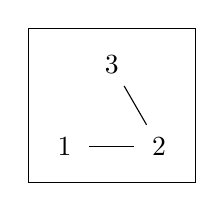
\begin{tikzpicture}[scale=.8, show background rectangle]
    \tikzstyle{every node} = [circle]
    \node (a) at (0,0) {1};
    \node (b) at +(0:1.5) {2};
    \node (c) at +(60:1.5) {3};
    \foreach \from/\to in {a/b, b/c}
      \draw (\from) -- (\to);
  \end{tikzpicture}
  \caption{Diagram for $G=(\set{1, 2, 3}, \set{(1,2), (2,1), (2,3), (3,2)})$}
  \label{fig:example-graph}
\end{figure}


All the results are from \cite{paper}.


\section{Graph Limits}
Explain graph limit in detail.
\subsection{Introduction}
Explain the space of graph limits here. 

$\Ug$ is the space of unlabeled graphs, and $\Ug[\infty] \coloneqq \Ug* \setminus \Ug$ is the space of proper graph limits.

\subsection{Random Graphs}
\begin{theorem}
  Let $(G_n | n \geq 1)$ be a sequence of random unlabeled graphs and assume that $v(G_n) \pconv \infty$. Then the following are equivalent, as $n \to \infty$.
  \begin{enumerate}
      \item $G_n \dconv \Gamma$ for some random $\Gamma \in \Ug*$
      \item For every finite family $F_1, F_2 \ldots, F_m$ of (non-random) graphs, the random variables $t(F, G_n)$ converge in distribution.
      \item For every (non-random) $F \in \Ug$, the random variables $t(F, G_n)$ converge in distribution.
      \item For every (non-random) $F \in \Ug$, the expectations $\Ex{t(F, G_n)}$ converge.
    \end{enumerate}
    If these properties hold, then the limits in (ii), (iii) and (iv) are $\left( (t(F_i, \Gamma) \right)_{i=1}^m$, $t(F, \Gamma)$ and $\Ex{t(F, \Gamma)}$, respectively. Furthermore, $\Gamma \in \Ug[\infty]$ a.s
  \label{thm:dconv-random-graphs}
\end{theorem}


\section{Exchangeable Random Graphs}
\subsection{Infinite Graphs}
Describe the space of infinite graphs and weak convergence there.

\begin{theorem}
   Let $\left( G_n \right)$ be a sequence of random graphs in $\Ug$ and assume that $v(G_n) \to \infty$. Then the following are equivalent.
  \begin{enumerate}
    \item $G_n \dconv \Gamma$ in $\Ug*$ for some random variable $\Gamma \in \Ug*$
    \item $\widehat{G_n} \dconv H$ in $\Lg$ for some random $H \in \Lg$
  \end{enumerate}
  If these hold, then $\Pb{\restr{H}{[k]} = F} = \Ex{t_{ind}(F, \Gamma)}$ for every $F \in \Lg[k]$. Furthermore, $\Gamma \in \Ug[\infty]$ a.s
   
  \label{thm:conv-to-infinite-graphs}
\end{theorem}

\printbibliography
\end{document}


